\documentclass[12pt,a4paper]{article}

% --- PAQUETES PRINCIPALES ---
\usepackage[utf8]{inputenc}
\usepackage[spanish,es-nodecimaldot]{babel}
\usepackage[left=2.5cm,right=2.5cm,top=2.5cm,bottom=2.5cm]{geometry}
\usepackage{graphicx}
\usepackage{xcolor}
\usepackage{hyperref}
\usepackage{booktabs}
\usepackage{enumitem}
\usepackage{fancyhdr}
\usepackage{titlesec}
\usepackage{caption}
\usepackage{float}
\usepackage{listings}
\usepackage{microtype}
\usepackage{array}

% --- RUTA DE GRÁFICOS ---
\graphicspath{{./}{Informe/}{./Informe/}}

% --- PALETA DE COLORES INSTITUCIONAL CUSCO REPORTA ---
\definecolor{cuscoGold}{HTML}{F9D276}
\definecolor{cuscoGoldDark}{HTML}{D4AF37}
\definecolor{cuscoCrimson}{HTML}{AD1D45}
\definecolor{cuscoWine}{HTML}{83142C}
\definecolor{cuscoMaroon}{HTML}{44000D}
\definecolor{darkText}{HTML}{2D3748}
\definecolor{lightGray}{HTML}{F7FAFC}
\definecolor{borderGray}{HTML}{E2E8F0}

% --- CONFIGURACIÓN DE HIPERVÍNCULOS ---
\hypersetup{
    colorlinks=true,
    linkcolor=cuscoWine,
    citecolor=cuscoCrimson,
    urlcolor=cuscoCrimson,
    pdftitle={Informe Técnico - Plataforma Web de Reportes e Incidencias Urbanas},
    pdfauthor={Villavicencio, Charalla, Supa},
    pdfsubject={Desarrollo de Software II - UNSAAC}
}

% --- FORMATO DE TÍTULOS ---
\titleformat{\section}
  {\normalfont\Large\bfseries\color{cuscoWine}}{\thesection}{1em}{}[\titlerule]
\titleformat{\subsection}
  {\normalfont\large\bfseries\color{cuscoCrimson}}{\thesubsection}{1em}{}
\titleformat{\subsubsection}
  {\normalfont\normalsize\bfseries\color{cuscoMaroon}}{\thesubsubsection}{1em}{}

% --- ENCABEZADOS Y PIES DE PÁGINA ---
\pagestyle{fancy}
\setlength{\headheight}{15pt}
\fancyhf{}
\fancyhead[L]{\small\color{gray}UNSAAC - Desarrollo de Software II}
\fancyhead[R]{\small\color{cuscoWine}\textbf{Cusco Reporta}}
\fancyfoot[C]{\thepage}
\renewcommand{\headrulewidth}{0.5pt}
\renewcommand{\footrulewidth}{0.5pt}

% --- CONFIGURACIÓN DE CÓDIGO FUENTE ---
\lstset{
    basicstyle=\ttfamily\footnotesize,
    backgroundcolor=\color{lightGray},
    keywordstyle=\color{cuscoCrimson}\bfseries,
    stringstyle=\color{cuscoWine},
    commentstyle=\color{gray}\itshape,
    numberstyle=\tiny\color{gray},
    numbers=left,
    stepnumber=1,
    numbersep=8pt,
    showstringspaces=false,
    breaklines=true,
    frame=lines,
    rulecolor=\color{borderGray},
    tabsize=2
}

\begin{document}

% ==============================================================================
% CARÁTULA OFICIAL (RÉPLICA EXACTA DEL FORMATO SOLICITADO)
% ==============================================================================
\begin{titlepage}
    \thispagestyle{empty}
    \centering
    \vspace*{-1.2cm}
    
    {\fontsize{15}{18}\selectfont \textbf{UNIVERSIDAD NACIONAL SAN ANTONIO ABAD DEL CUSCO}\par}
    \vspace{0.35cm}
    {\fontsize{10.5}{13.5}\selectfont \textbf{FACULTAD DE INGENIERÍA ELÉCTRICA, ELECTRÓNICA, INFORMÁTICA, Y MECÁNICA}\par}
    
    \vspace{0.7cm}
    
    % Logos oficiales centrados
    
\includegraphics[width=4.3cm]{logo_unsaac.png}\par
    \vspace{0.45cm}
    
\includegraphics[width=3.7cm]{logo_fiis.png}\par
    
    \vspace{0.75cm}
    
    % Doble línea y texto de Escuela Profesional
    \rule{\linewidth}{1.8pt}\par
    \vspace{0.18cm}
    {\fontsize{11}{14}\selectfont \textbf{ESCUELA PROFESIONAL DE INGENIERÍA INFORMÁTICA Y DE SISTEMAS}\par}
    \vspace{0.18cm}
    \rule{\linewidth}{1.2pt}\par
    
    \vspace{0.75cm}
    
    % Título del proyecto
    {\fontsize{14}{18}\selectfont \textbf{Plataforma Web de Reportes e Incidencias Urbanas}\par}
    
    \vspace{1.1cm}
    
    % Datos informativos
    \begin{flushleft}
    \fontsize{11}{15}\selectfont
    \textbf{Asignatura:} Desarrollo de Software II\\[0.25cm]
    \textbf{Docente:} Hans Harley Ccacyahuillca Bejar\\[0.25cm]
    \textbf{Integrantes:}\\[0.15cm]
    \hspace*{0.5cm} -- Edu Piero Villavicencio Seguil\\
    \hspace*{0.5cm} -- Gianfranco Charalla Ccama\\
    \hspace*{0.5cm} -- Yeferson Supa Cusipaucar\\[0.35cm]
    \textbf{Fecha:} 28/10/2026
    \end{flushleft}
    
    \vfill
\end{titlepage}

% ==============================================================================
% TABLA DE CONTENIDOS
% ==============================================================================
\newpage
\pagenumbering{roman}
\tableofcontents
\newpage
\pagenumbering{arabic}

% ==============================================================================
% RESUMEN EJECUTIVO
% ==============================================================================
\section*{Resumen Ejecutivo}
\addcontentsline{toc}{section}{Resumen Ejecutivo}

El presente informe técnico documenta el diseño, desarrollo e implementación integral de la plataforma web \textbf{Cusco Reporta}, una solución tecnológica orientada a la gestión inteligente, georreferenciada y participativa de incidencias urbanas en la provincia de Cusco. 

La plataforma aborda deficiencias críticas en la interacción entre la ciudadanía y las dependencias de la Municipalidad Provincial del Cusco, permitiendo registrar problemas de infraestructura pública (alumbrado deficiente, cúmulos de basura, vías deterioradas, áreas verdes, fugas de agua y seguridad ciudadana) con captura automática de coordenadas GPS y fotografía de evidencia. 

Construida bajo una arquitectura desacoplada basada en micro-servicios y clientes SPA (\textit{Single Page Application}), el sistema integra React 18, Vite 7, Node.js con Express, una base de datos relacional MySQL optimizada, y librerías cartográficas como Leaflet. Asimismo, se implementó un sistema de diseño propio basado en la identidad cromática cusqueña, un selector ergonómico de categorías en cuadrícula estática sin desplazamiento horizontal, un módulo de atención directa vía WhatsApp, una línea de tiempo progresiva de cuatro etapas y un directorio telefónico de emergencias.

\vspace{0.5cm}
\noindent\textbf{Palabras clave:} Desarrollo Web, React, Node.js, Incidencias Urbanas, Georreferenciación GPS, Cusco Reporta, Participación Ciudadana, Leaflet, MySQL.

% ==============================================================================
% 1. INTRODUCCIÓN Y PROBLEMÁTICA
% ==============================================================================
\section{Introducción y Problemática}

\subsection{Contexto y Planteamiento del Problema}
La provincia del Cusco, como centro histórico, administrativo y turístico de gran relevancia internacional, enfrenta retos diarios en el mantenimiento y conservación de sus servicios básicos e infraestructura pública. Problemas como postes de alumbrado sin funcionamiento, buzones de desagüe sin tapa, acumulación irregular de residuos sólidos en esquinas patrimoniales y baches en arterias de alto tránsito suelen reportarse mediante trámites burocráticos engorrosos en mesa de partes física, o bien se difunden informalmente en redes sociales sin canalización estructurada.

Esta desarticulación genera:
\begin{itemize}[leftmargin=*]
    \item \textbf{Tiempos de respuesta prolongados:} La falta de georreferenciación exacta dificulta que las cuadrillas de obras o limpieza localicen el punto del incidente.
    \item \textbf{Opacidad en el seguimiento:} El vecino no cuenta con un mecanismo en tiempo real para conocer si su reclamo fue evaluado, derivado o concluido.
    \item \textbf{Carencia de métricas consolidadas:} Las gerencias municipales carecen de tableros estadísticos confiables para priorizar recursos e intervenciones operativas.
\end{itemize}

\subsection{Justificación Tecnológica y Social}
El proyecto \textbf{Cusco Reporta} nace como respuesta académica y tecnológica dentro de la asignatura de \textit{Desarrollo de Software II} en la UNSAAC. Permite cerrar la brecha entre el ciudadano y la municipalidad a través de una aplicación web moderna, accesible y adaptativa, disponible las 24 horas del día.

\subsection{Objetivos del Proyecto}
\subsubsection{Objetivo General}
Desarrollar, desplegar y validar una plataforma web integral para el registro, geolocalización, canalización y resolución de incidencias urbanas en la provincia del Cusco, garantizando trazabilidad y soporte multirrol.

\subsubsection{Objetivos Específicos}
\begin{enumerate}[leftmargin=*]
    \item Implementar un sistema de autenticación y autorización robusto basado en Control de Acceso Basado en Roles (RBAC: Ciudadano, Autoridad y Administrador).
    \item Diseñar una interfaz de usuario accesible y moderna, utilizando la paleta institucional cusqueña y navegación por pestañas ergonómicas sin desplazamiento horizontal excesivo.
    \item Incorporar capacidades de geolocalización satelital (GPS HTML5) y mapas interactivos mediante la librería Leaflet y OpenStreetMap.
    \item Proveer canales de interacción directa, incluyendo un botón de WhatsApp vinculado con agentes especializados y un directorio de emergencias de Cusco.
    \item Proporcionar trazabilidad transparente mediante una línea de tiempo (\textit{stepper}) visual del ciclo de vida de cada reporte.
\end{enumerate}

% ==============================================================================
% 2. ARQUITECTURA DEL SISTEMA Y PILA TECNOLÓGICA
% ==============================================================================
\section{Arquitectura del Sistema y Pila Tecnológica}

\subsection{Arquitectura Cliente-Servidor Desacoplada}
El sistema adopta el patrón arquitectónico cliente-servidor desacoplado mediante una \textbf{API RESTful}, lo que asegura independencia de capas, alta mantenibilidad y escalabilidad a futuras aplicaciones móviles nativas.

\begin{figure}[H]
    \centering
    \begin{center}
    \setlength{\fboxsep}{10pt}
    \setlength{\fboxrule}{1pt}
    \fcolorbox{cuscoWine}{lightGray}{
        \begin{minipage}{0.9\textwidth}
        \centering
        \textbf{\color{cuscoWine}DIAGRAMA DE ARQUITECTURA DEL SISTEMA}\\[0.3cm]
        \textbf{Capa de Presentación (Frontend):} React 18 + Vite + Context API + Leaflet\\
        $\updownarrow$ \textit{Peticiones Asíncronas HTTP/REST (JSON / Multipart)}\\
        \textbf{Capa Lógica y Negocio (Backend API):} Node.js + Express + JWT + Multer\\
        $\updownarrow$ \textit{Controlador de Conexión Pool (mysql2)}\\
        \textbf{Capa de Persistencia (Base de Datos):} MySQL 8.0 (Tablas Relacionales, Índices, Vistas)
        \end{minipage}
    }
    \end{center}
    \caption{Esquema conceptual de la arquitectura en tres capas de Cusco Reporta.}
    \label{fig:arquitectura}
\end{figure}

\subsection{Pila Tecnológica Seleccionada}

\subsubsection{Frontend (Cliente Web)}
\begin{itemize}[leftmargin=*]
    \item \textbf{React 18.2:} Biblioteca declarativa para la construcción de interfaces de usuario modulares y reactivas.
    \item \textbf{Vite 7.1:} Entorno de construcción ultrarrápido con \textit{Hot Module Replacement} (HMR), optimizando los tiempos de transpilación y empaquetado.
    \item \textbf{Context API:} Manejo de estados globales sin sobrecarga de dependencias externas:
        \begin{itemize}
            \item \texttt{AuthContext}: Sesión, token JWT y perfil del usuario autenticado.
            \item \texttt{ReportContext}: Caché y sincronización de reportes, estadísticas y filtros.
            \item \texttt{ToastContext}: Notificaciones emergentes accesibles y reactivas.
        \end{itemize}
    \item \textbf{Leaflet 1.9.4:} Motor cartográfico ligero para el renderizado de mapas interactivos OpenStreetMap con marcadores temáticos.
    \item \textbf{Axios 1.6:} Cliente HTTP para la comunicación con la API, configurado con interceptores para encabezados de autorización.
\end{itemize}

\subsubsection{Backend (Servidor de Aplicaciones y API)}
\begin{itemize}[leftmargin=*]
    \item \textbf{Node.js \& Express 4.18:} Entorno de ejecución asíncrono y framework minimalista para endpoints REST.
    \item \textbf{jsonwebtoken (JWT):} Emisión y verificación de tokens criptográficos con expiración programada.
    \item \textbf{bcryptjs:} Algoritmo de hashing salteado de contraseñas para resguardar las credenciales ciudadanas.
    \item \textbf{multer:} Middleware para gestión y almacenamiento seguro de evidencias fotográficas en disco (\textit{multipart/form-data}).
    \item \textbf{mysql2:} Driver optimizado con soporte para consultas parametrizadas seguras (\textit{prepared statements}) y \textit{connection pooling}.
\end{itemize}

\subsubsection{Identidad Visual y Sistema de Diseño}
La identidad cromática se construyó con base en la herencia andina e institucional de la Municipalidad Provincial del Cusco:
\begin{itemize}[leftmargin=*]
    \item \textbf{Dorado Inti (\#F9D276):} Acentos principales, estados activos, botones primarios y encabezados jerárquicos.
    \item \textbf{Carmesí Andino (\#AD1D45):} Botones secundarios, insignias de estado en proceso y alertas operativas.
    \item \textbf{Vino Tinto Imperial (\#83142C):} Superficies de tarjetas, modales y barras de herramientas.
    \item \textbf{Granate Medianoche (\#44000D):} Fondos oscuros con acabado de cristal templado (\textit{glassmorphism}) y degradados radiales.
    \item \textbf{Tipografías Oficiales:} \textit{Outfit} (títulos modernos), \textit{Plus Jakarta Sans} (lectura continua y formularios) y \textit{Cinzel} (acabados protocolares e históricos).
\end{itemize}

% ==============================================================================
% 3. MODELADO DE DATOS Y SEGURIDAD
% ==============================================================================
\section{Modelado de Datos y Seguridad}

\subsection{Esquema Relacional de Base de Datos}
La base de datos relacional \texttt{santiago\_reporta} está optimizada para la integridad referencial y alto rendimiento en consultas de búsqueda y conteo.

\begin{table}[H]
\centering
\small
\caption{Estructura de las tablas principales de la base de datos.}
\label{tab:tablas_bd}
\begin{tabular}{lllp{6.5cm}}
\toprule
\textbf{Tabla} & \textbf{Campo Clave} & \textbf{Tipo de Dato} & \textbf{Descripción y Restricción} \\
\midrule
\texttt{users} & \texttt{id} & INT (PK, AI) & Identificador único del usuario. \\
 & \texttt{email} & VARCHAR(100) & Correo electrónico único con índice indexado. \\
 & \texttt{password} & VARCHAR(255) & Hash seguro generado mediante bcrypt. \\
 & \texttt{role} & ENUM & Rol: \texttt{'citizen'}, \texttt{'authority'}, \texttt{'admin'}. \\
\midrule
\texttt{reports} & \texttt{id} & INT (PK, AI) & Identificador numérico interno. \\
 & \texttt{code} & VARCHAR(20) & Código legible único (ej. RPT-001, RPT-002). \\
 & \texttt{title} & VARCHAR(200) & Resumen textual de la incidencia. \\
 & \texttt{type} & ENUM & Tipo: vías, alumbrado, basura, parques, agua, seguridad, otros. \\
 & \texttt{priority} & ENUM & Nivel de urgencia: baja, media, alta. \\
 & \texttt{status} & ENUM & Estado: \texttt{'pending'}, \texttt{'progress'}, \texttt{'resolved'}. \\
 & \texttt{citizen\_id} & INT (FK) & Referencia a \texttt{users(id)} con borrado en cascada. \\
 & \texttt{latitude} & DECIMAL(10,8) & Coordenada GPS latitudinal. \\
 & \texttt{longitude} & DECIMAL(11,8) & Coordenada GPS longitudinal. \\
 & \texttt{photo\_url} & VARCHAR(255) & Ruta relativa a la fotografía subida. \\
\midrule
\texttt{report\_updates} & \texttt{id} & INT (PK, AI) & Historial de auditoría de cada actualización. \\
 & \texttt{report\_id} & INT (FK) & Incidencia asociada. \\
 & \texttt{user\_id} & INT (FK) & Autoridad municipal que ejecuta la modificación. \\
 & \texttt{new\_status} & ENUM & Estado asignado tras la intervención. \\
 & \texttt{comment} & TEXT & Bitácora técnica y observaciones operativas. \\
\bottomrule
\end{tabular}
\end{table}

\subsection{Estrategia de Seguridad y Políticas CORS}
\begin{itemize}[leftmargin=*]
    \item \textbf{CORS Dinámico:} El servidor implementa una política basada en expresiones regulares para validar orígenes locales (\texttt{localhost} y \texttt{127.0.0.1} en cualquier puerto dinámico asignado por Vite), evitando bloqueos durante el flujo de desarrollo.
    \item \textbf{Control de Acceso Basado en Roles (RBAC):} Rutas protegidas mediante middlewares en Express (\texttt{authMiddleware.js}) que decodifican el token JWT del encabezado \texttt{Authorization: Bearer <token>} y validan los privilegios de ejecución.
    \item \textbf{Sanitización de Consultas:} Empleo estricto de sentencias SQL preparadas con placeholders (\texttt{?}) para mitigar vulnerabilidades de inyección SQL (SQLi).
\end{itemize}

% ==============================================================================
% 4. MÓDULOS Y FUNCIONALIDADES IMPLEMENTADAS
% ==============================================================================
\section{Módulos y Funcionalidades Implementadas}

\subsection{Módulo de Inicio y Autenticación Unificada (Home)}
Punto de entrada institucional con diseño acogedor e informativo. Cuenta con:
\begin{itemize}[leftmargin=*]
    \item Resumen de las virtudes del sistema y panel fotográfico del Cusco histórico.
    \item Métricas globales en tiempo real que informan al visitante sobre la actividad municipal.
    \item Formulario de acceso único (\textit{Login / Registro}) que redirige dinámicamente según el rol (\texttt{citizen} $\rightarrow$ Portal Ciudadano, \texttt{authority} $\rightarrow$ Panel de Autoridad, \texttt{admin} $\rightarrow$ Panel de Administración).
\end{itemize}

\subsection{Módulo del Ciudadano (Portal de Reportes)}
Diseñado bajo principios de usabilidad ergonómica:
\begin{itemize}[leftmargin=*]
    \item \textbf{Selector de Categorías en Doble Fila (Estilo Dribbble):} Disposición en cuadrícula estática de 4 columnas por 2 filas que elimina todo desplazamiento horizontal en pantalla:
    \begin{center}
    \small
    \fbox{\textbf{Fila 1:}} [Todas] \quad [Alumbrado Público] \quad [Limpieza y Basura] \quad [Vías y Pistas]\\
    \vspace{0.15cm}
    \fbox{\textbf{Fila 2:}} [Parques y Áreas Verdes] \quad [Agua y Alcantarillado] \quad [Seguridad y Orden] \quad [Otros Reclamos]
    \end{center}
    Al hacer clic en cualquier píldora, esta se ilumina en dorado institucional y preconfigura de inmediato el formulario inferior.
    
    \item \textbf{Formulario de Reporte Urbano Inteligente:}
    \begin{itemize}
        \item Letrero identificativo con indicación de la categoría activa.
        \item Sugerencias rápidas automáticas (+ Poste apagado, + Cables caídos, + Baches, etc.) que se insertan en un solo clic.
        \item Captura de coordenadas GPS nativa mediante la API Geolocation del navegador.
        \item Carga y previsualización de evidencia fotográfica con opción de reemplazo.
    \end{itemize}

    \item \textbf{Historial Personal de Incidencias:}
    Visualización filtrable por categoría con contadores específicos y badges de estado (\textit{Pendiente, En Proceso, Resuelto}).
\end{itemize}

\subsection{Módulo de Asistencia Directa y Directorio de Emergencias}
\begin{itemize}[leftmargin=*]
    \item \textbf{Canal de WhatsApp Simplificado:} Widget flotante accesible con botón verde esmeralda y modal unificado que conecta al ciudadano con el enlace oficial de atención:
    \begin{center}
    \url{https://api.whatsapp.com/send/?phone=51918643261&text&type=phone_number&app_absent=0}
    \end{center}
    \item \textbf{Línea de Tiempo Visual (\textit{Stepper} Progresivo):} Integrada en cada reporte individual para desglosar el avance municipal en 4 hitos:
    \begin{enumerate}
        \item \textit{Reporte Registrado:} Generación de código y fecha de registro.
        \item \textit{Evaluación Técnica:} Validación y derivación a la gerencia respectiva.
        \item \textit{Cuadrilla Asignada:} Personal técnico en campo atendiendo la zona.
        \item \textit{Incidencia Resuelta:} Cierre de orden y conformidad municipal.
    \end{enumerate}
    \item \textbf{Directorio Telefónico de Emergencias de Cusco:} Listado interactivo de las 8 centrales de auxilio (Serenazgo, Policía 105, Bomberos 116, SAMU 106, SedaCusco, Electro Sur Este, Municipalidad y Hospital Regional) con botones de llamada directa (\texttt{tel:}) y copiado instantáneo al portapapeles.
\end{itemize}

\subsection{Módulo de la Autoridad Municipal}
Herramienta operativa para funcionarios y cuadrillas:
\begin{itemize}[leftmargin=*]
    \item Panel de filtrado rápido por estado de atención.
    \item Botones de acción directa: \textit{"Iniciar Atención"} (cambio a En Proceso) y \textit{"Finalizar"} (cambio a Resuelto).
    \item Enlace directo a Google Maps para inspección satelital de la ubicación reportada.
    \item Visualización de evidencia fotográfica adjunta en modal emergente.
\end{itemize}

\subsection{Módulo del Administrador del Sistema}
Panel de gobernanza y control:
\begin{itemize}[leftmargin=*]
    \item Auditoría de usuarios registrados con visualización de fecha de alta.
    \item Asignación y revocación dinámica de privilegios de autoridad en tiempo real.
    \item Bloqueo de auto-degradación de cuentas administradoras maestras.
\end{itemize}

% ==============================================================================
% 5. EVIDENCIAS Y VISTAS DEL SISTEMA (CAPTURAS PRINCIPALES)
% ==============================================================================
\newpage
\section{Evidencias y Vistas del Sistema}

A continuación, se presentan y describen detalladamente las cuatro capturas principales del aplicativo web en ejecución, que demuestran la operatividad de los módulos descritos.

\subsection{Vista Principal e Inicio de Sesión (Home)}
La Figura~\ref{fig:captura_home} ilustra la pantalla inicial de bienvenida. En ella se evidencia el diseño con paleta institucional cusqueña, la barra superior con escudo oficial, el lema institucional en tipografía caligráfica, la imagen panorámica de la ciudad y el formulario interactivo de acceso al sistema con selector de rol.

\begin{figure}[H]
    \centering
    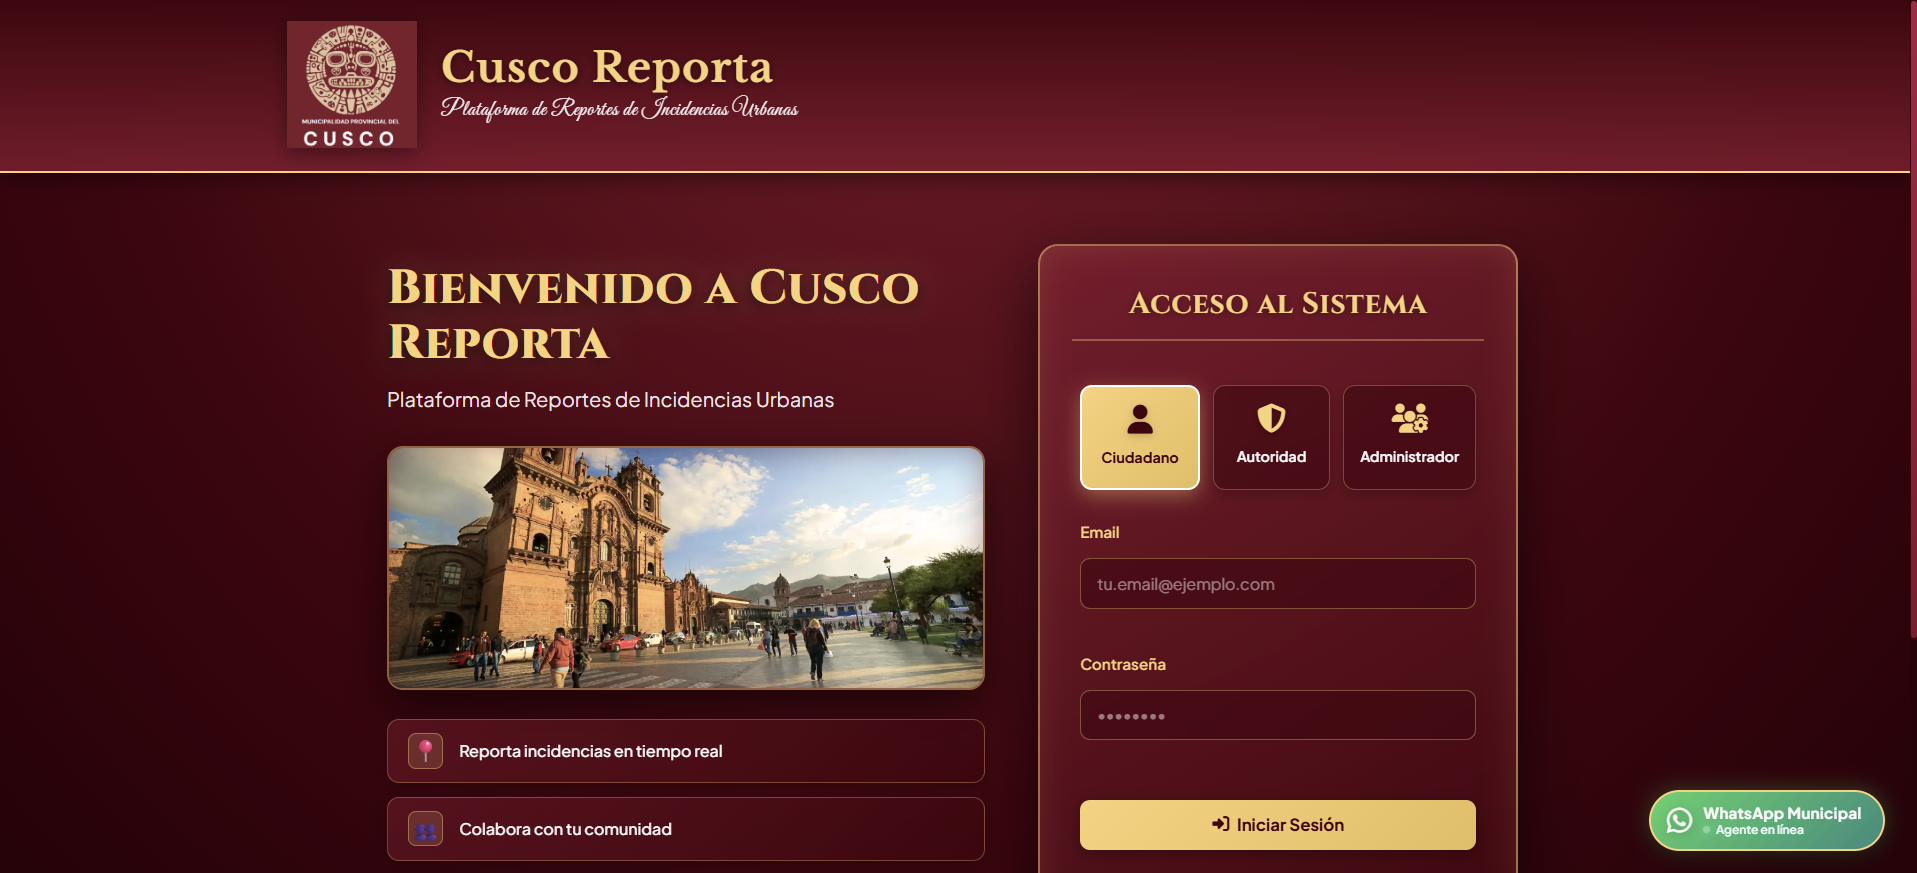
\includegraphics[width=0.96\textwidth]{Home.png}
    \caption{Pantalla de Inicio (\textit{Home}): bienvenida institucional, métricas públicas y formulario de autenticación.}
    \label{fig:captura_home}
\end{figure}

\subsection{Portal del Ciudadano y Formulario de Incidencias}
La Figura~\ref{fig:captura_ciudadano} muestra la interfaz de trabajo del vecino cusqueño autenticado. Se aprecian las mini-métricas personales en la cabecera, la barra de selección de categorías organizada exactamente en 2 filas sin desplazamiento horizontal, y el letrero \textit{"Formulario de Reporte Urbano"} sincronizado con la categoría seleccionada, junto al botón flotante de WhatsApp en la esquina inferior.

\begin{figure}[H]
    \centering
    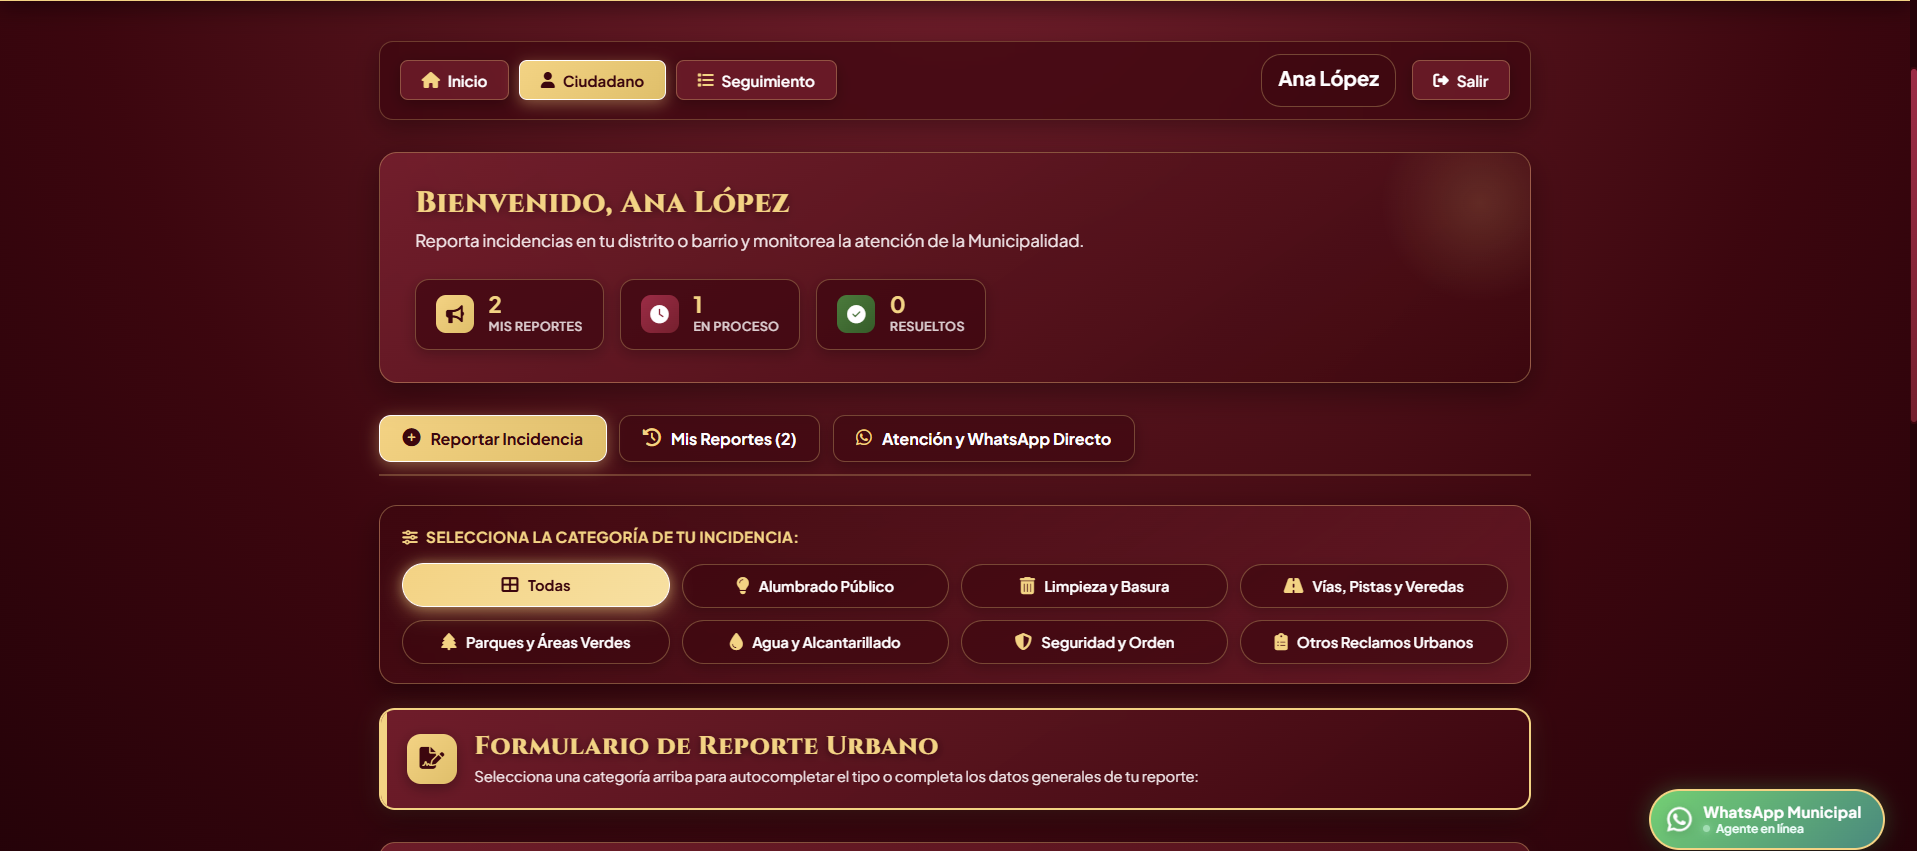
\includegraphics[width=0.96\textwidth]{Ciudadano.png}
    \caption{Portal del Ciudadano: mini-métricas personales, selector de categorías en dos filas y formulario inteligente.}
    \label{fig:captura_ciudadano}
\end{figure}

\subsection{Panel de Gestión de la Autoridad Municipal}
La Figura~\ref{fig:captura_autoridad} exhibe la vista de gestión para los inspectores y autoridades municipales. Permite auditar el inventario de reportes ciudadanos, visualizar la fotografía de evidencia, consultar coordenadas geográficas y accionar los controles de transición de estado (\textit{Iniciar atención} y \textit{Resolver}).

\begin{figure}[H]
    \centering
    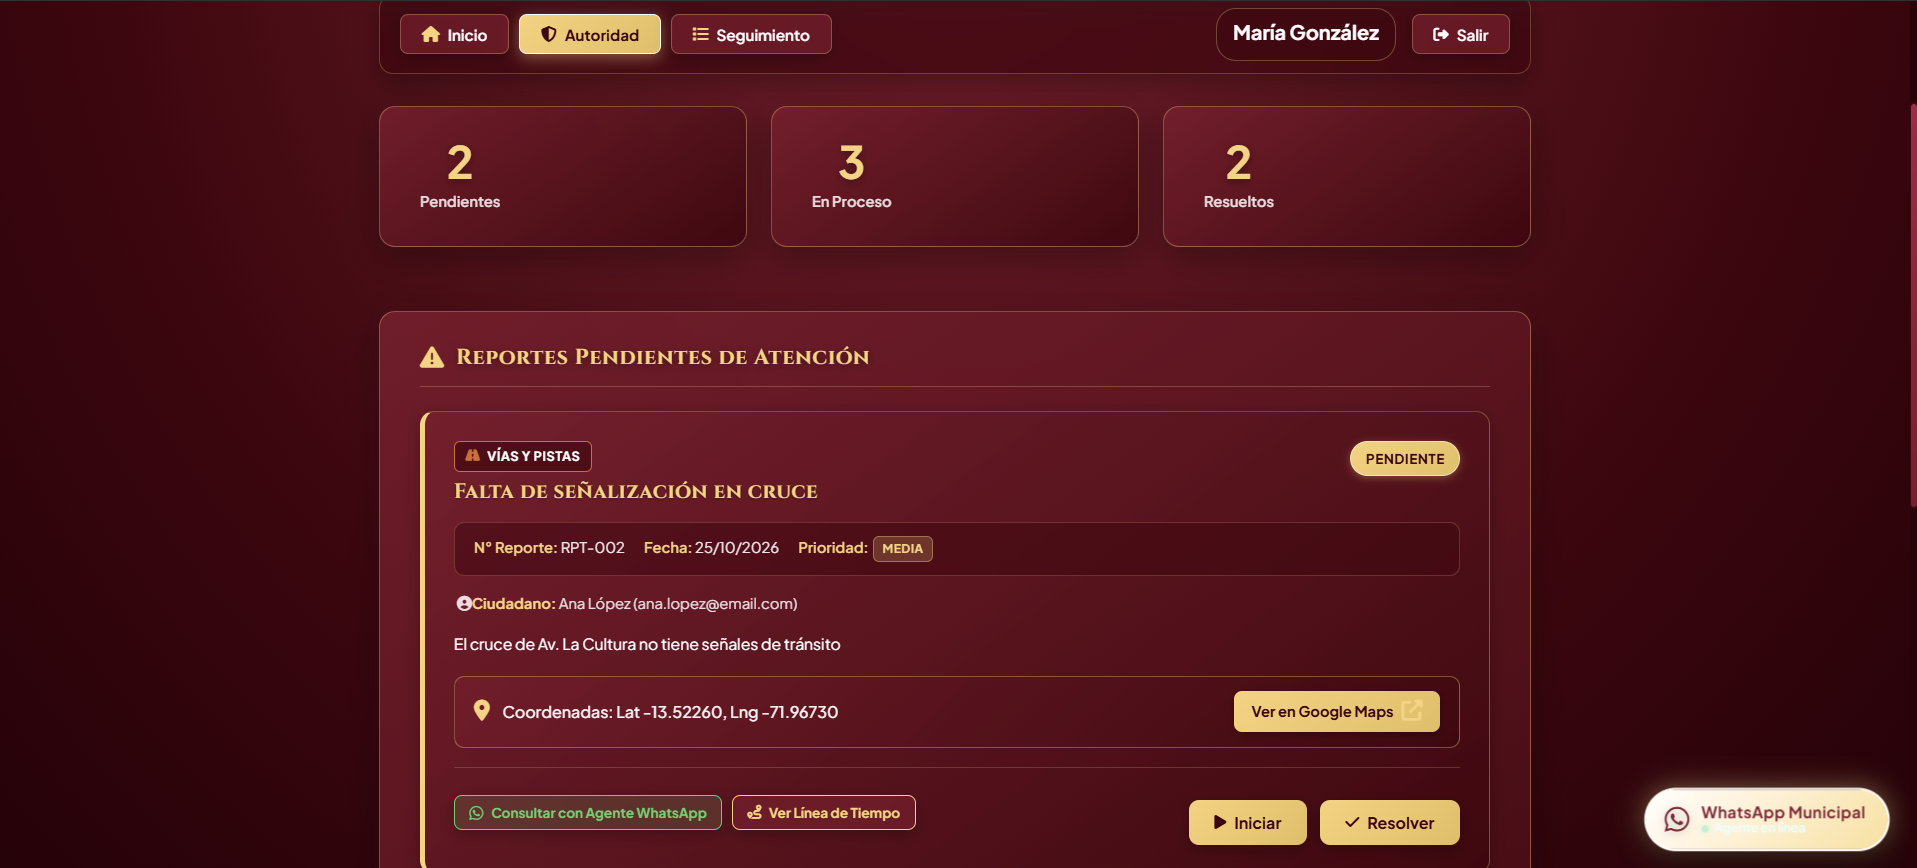
\includegraphics[width=0.96\textwidth]{Autoridad.png}
    \caption{Panel de Autoridad: gestión del ciclo de vida de incidencias, evidencia fotográfica y controles de actualización.}
    \label{fig:captura_autoridad}
\end{figure}

\subsection{Panel de Administración y Control de Usuarios}
La Figura~\ref{fig:captura_administrador} presenta la vista de administración global. Se listan todos los usuarios de la base de datos con sus respectivos roles y marcas temporales, permitiendo promover usuarios comunes a autoridades municipales o revocar privilegios con actualización en caliente.

\begin{figure}[H]
    \centering
    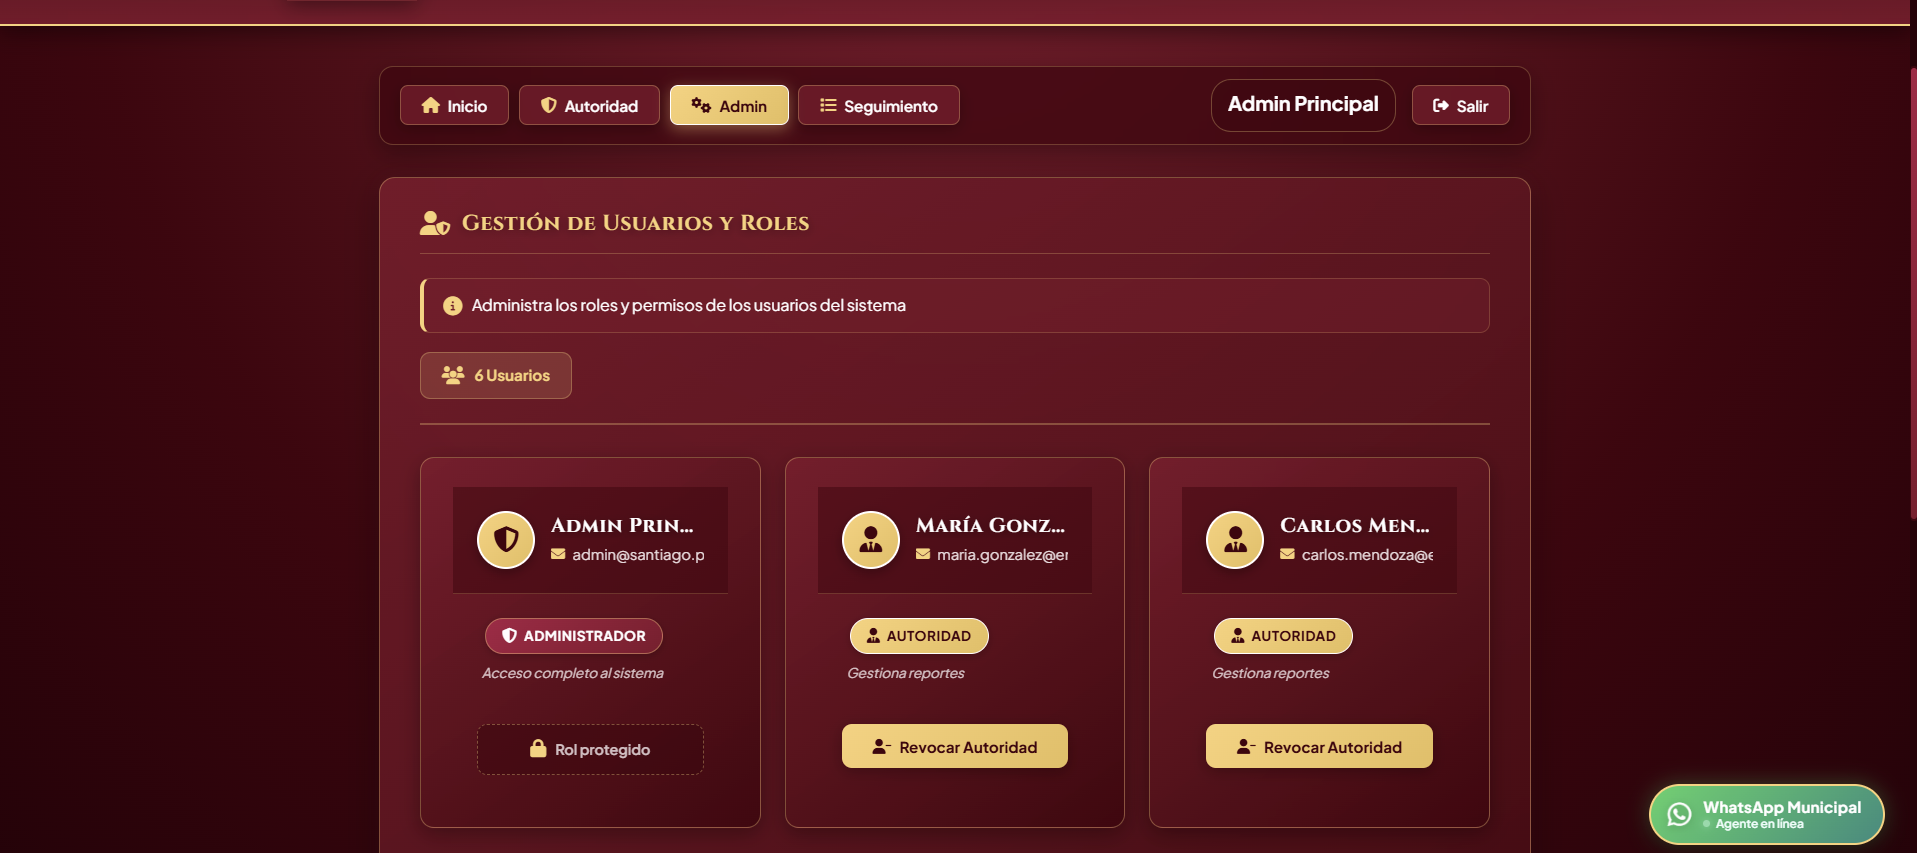
\includegraphics[width=0.96\textwidth]{Administrador.png}
    \caption{Panel de Administración: gestión de usuarios, asignación de roles y control de privilegios en el sistema.}
    \label{fig:captura_administrador}
\end{figure}

% ==============================================================================
% 6. CONCLUSIONES Y TRABAJO FUTURO
% ==============================================================================
\section{Conclusiones y Trabajo Futuro}

\subsection{Conclusiones}
\begin{enumerate}[leftmargin=*]
    \item Se completó con éxito el desarrollo e integración de la plataforma web \textbf{Cusco Reporta}, satisfaciendo los requerimientos funcionales, pedagógicos y de diseño establecidos para la asignatura de \textit{Desarrollo de Software II}.
    \item La separación arquitectónica entre React en el frontend y Node.js/Express en el backend demostró ser una solución robusta, facilitando la depuración modular y garantizando un tiempo de carga optimizado gracias al bundler Vite.
    \item La adopción del sistema de diseño propio basado en la cromática andino-cusqueña otorgó identidad institucional y prestigio visual a la plataforma, superando la apariencia genérica de plantillas convencionales.
    \item Las innovaciones de usabilidad introducidas —el selector de categorías en dos filas fijas sin scroll horizontal, la línea de tiempo progresiva, el botón simplificado de WhatsApp y el directorio telefónico de emergencias— mejoran sustancialmente la experiencia del ciudadano al registrar y consultar incidencias.
\end{enumerate}

\subsection{Trabajo Futuro y Recomendaciones}
\begin{itemize}[leftmargin=*]
    \item \textbf{Integración de un Mapa de Incidencias Personales (Portal Ciudadano):} Incorporar una vista cartográfica interactiva dentro de la sección del ciudadano donde se visualicen georreferenciados todos los reportes emitidos por el usuario, permitiendo filtrar sus incidencias por estado y verificar visualmente su ubicación en el mapa de la ciudad del Cusco.
    \item \textbf{Integración de un Mapa Centralizado de Incidencias Urbanas (Panel de Autoridad):} Desarrollar un mapa geoespacial consolidado para el perfil de Autoridad Municipal que despliegue la totalidad de incidencias generadas por la ciudadanía, con filtros por sector, niveles de urgencia y mapas de calor que faciliten la planificación y despacho eficiente de las cuadrillas operativas.
    \item \textbf{Simplificación y Accesibilidad Universal de la Interfaz:} Continuar optimizando y depurando la interfaz gráfica de usuario para maximizar la simplicidad y ergonomía del flujo de reporte, garantizando que cualquier tipo de ciudadano, sin importar su nivel de alfabetización digital o edad, pueda reportar un problema urbano de manera rápida, clara y sin fricciones.
    \item \textbf{Autenticación Directa mediante Cuenta de Google (OAuth 2.0):} Implementar el inicio de sesión federado con Google (*Sign in with Google*), permitiendo a los vecinos autenticarse de forma instantánea y segura sin necesidad de completar formularios manuales de registro ni memorizar nuevas credenciales de acceso.
\end{itemize}

% ==============================================================================
% REFERENCIAS BIBLIOGRÁFICAS
% ==============================================================================
\newpage
\begin{thebibliography}{99}
\bibitem{react}
Facebook Open Source. (2024). \textit{Documentación Oficial de React 18}. Recuperado de: \url{https://react.dev/}

\bibitem{express}
OpenJS Foundation. (2024). \textit{Express - Node.js web application framework}. Recuperado de: \url{https://expressjs.com/}

\bibitem{mysql}
Oracle Corporation. (2024). \textit{MySQL 8.0 Reference Manual}. Recuperado de: \url{https://dev.mysql.com/doc/}

\bibitem{leaflet}
Agafonkin, V. (2024). \textit{Leaflet: an open-source JavaScript library for mobile-friendly interactive maps}. Recuperado de: \url{https://leafletjs.com/}

\bibitem{pressman}
Pressman, R. S., \& Maxim, B. R. (2020). \textit{Ingeniería del Software: Un Enfoque Práctico} (8va ed.). McGraw-Hill Interamericana.

\bibitem{sommerville}
Sommerville, I. (2019). \textit{Ingeniería de Software} (10ma ed.). Pearson Educación.
\end{thebibliography}

\end{document}
